\documentclass[10pt]{article}
\usepackage[margin=0.8in]{geometry}
\usepackage[utf8]{inputenc}
\usepackage[T1]{fontenc}
\usepackage{graphicx}
\usepackage[export]{adjustbox}
\usepackage{amsmath}
\usepackage{amsfonts}
\usepackage{amssymb}
\usepackage[version=4]{mhchem}
\usepackage{stmaryrd}
\usepackage{bbold}
\usepackage{fixltx2e}
\usepackage{caption}
\usepackage{mathtools}
\usepackage[parfill]{parskip}
\usepackage{float}
\usepackage{amsmath}
\usepackage{amssymb}

\begin{document}



\title{Lecture 13:  Singularity and Redundancy}
\date{Sep. 28, 2023}
\author{Wanxin Jin}
\maketitle



The Jacobian of a robot arm defines

$$
\boldsymbol{v}_{e}=\boldsymbol{J}(\boldsymbol{q}) \dot{\boldsymbol{q}}
$$

between  joint velocity $\dot{\boldsymbol{q}}$ and the end-effector velocity $\boldsymbol{v}_{e}=\left[\begin{array}{ll}\dot{\boldsymbol{p}}_{e}^{T} & \boldsymbol{\omega}_{e}^{T}\end{array}\right]^{T}$. Jacobian is a function of the configuration $\boldsymbol{q}$; those configurations at which $\boldsymbol{J}$ is rank-deficient are termed kinematic Singularities. Why we need to pay attention to kinematic Singularities?

(a) Singularities represent configurations at which mobility of the manipulator is reduced

(b) When the manipulator is at a singularity, infinite solutions to IK may exist.

(c) Near a singularity, small velocities in the operational space may cause large velocities in the joint space.








\section{Singularity Decoupling}
Computation of kinematic singularities via the Jacobian determinant may be tedious and of no easy solution for complex structures of manipulators. For manipulators having a spherical wrist, it is possible to split the problem of singularity computation into two separate problems: (1) computation of arm singularities resulting from the first 3 or more links, and (2) computation of wrist singularities resulting from the wrist joints.



Consider a $6$-DoF manipulator, where the outer 3 joints are all revolute (e.g., a spherical wrist), as shown for the Stanford Manipulator. 

\begin{figure}[H]
    \centering
    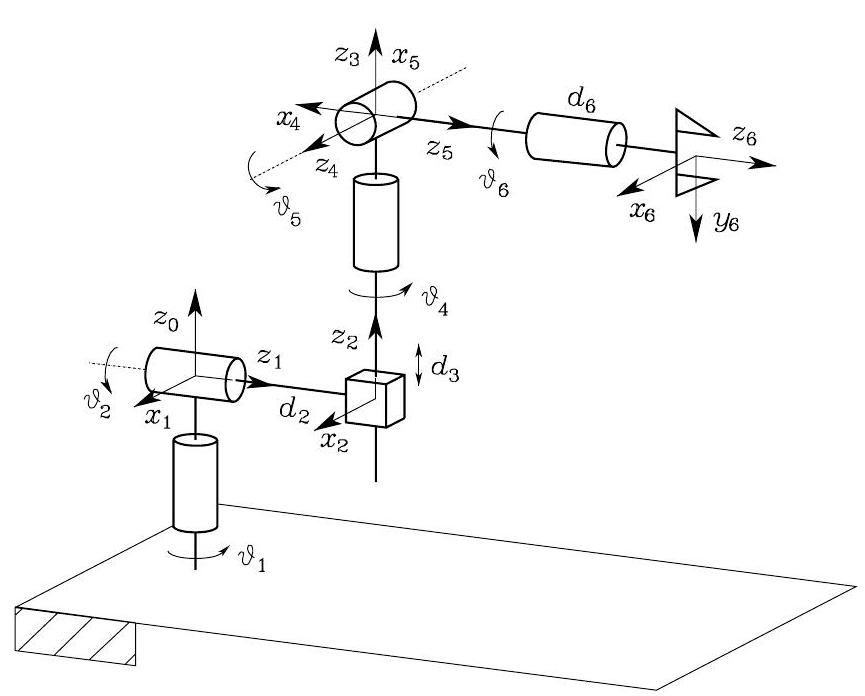
\includegraphics[max width=0.45\textwidth]{kinematics/Stanford_manipulator.jpg}
    \label{c1.l2.fig.Stanford}
\end{figure}



The Jacobian can be partitioned into $(2 \times 2)$ block matrix

$$
\boldsymbol{J}=\left[\begin{array}{ll}
\boldsymbol{J}_{11} & \boldsymbol{J}_{12} \\
\boldsymbol{J}_{21} & \boldsymbol{J}_{22}
\end{array}\right]
$$

with 

$$
\begin{gathered}
\boldsymbol{J}_{11}=\left[\begin{array}{ccc}
\boldsymbol{z}_{0} \times\left(\boldsymbol{p}_{e}-\boldsymbol{p}_{0}\right) & \boldsymbol{z}_{1} \times\left(\boldsymbol{p}_{e}-\boldsymbol{p}_{1}\right) & \boldsymbol{z}_{2} 
\end{array}\right] \\
\boldsymbol{J}_{21}=\left[\begin{array}{lll}
\boldsymbol{z}_{0} & \boldsymbol{z}_{1} & \boldsymbol{0}
\end{array}\right] .\\
\boldsymbol{J}_{12}=\left[\begin{array}{ccc}
\boldsymbol{z}_{3} \times\left(\boldsymbol{p}_{e}-\boldsymbol{p}_{3}\right) & \boldsymbol{z}_{4} \times\left(\boldsymbol{p}_{e}-\boldsymbol{p}_{4}\right) & \boldsymbol{z}_{5} \times\left(\boldsymbol{p}_{e}-\boldsymbol{p}_{5}\right)
\end{array}\right] \\
\boldsymbol{J}_{22}=\left[\begin{array}{lll}
\boldsymbol{z}_{3} & \boldsymbol{z}_{4} & \boldsymbol{z}_{5}
\end{array}\right] .
\end{gathered}
$$

By conducting row operations on the above Jacobian Matrix $\boldsymbol{J}$ (note that row operations maintain the matrix rank), we have obtained

$$
\boldsymbol{\Bar{J}}=\left[\begin{array}{ll}
\boldsymbol{\bar{J}}_{11} & \boldsymbol{0} \\
\boldsymbol{\bar{J}}_{21} & \boldsymbol{\bar{J}}_{22}
\end{array}\right]
$$


$$
\begin{gathered}
\boldsymbol{\bar{J}}_{11}=\left[\begin{array}{ccc}
\boldsymbol{z}_{0} \times\left(\boldsymbol{p}_{3}-\boldsymbol{p}_{0}\right) & \boldsymbol{z}_{1} \times\left(\boldsymbol{p}_{3}-\boldsymbol{p}_{1}\right) & \boldsymbol{z}_{2}
\end{array}\right] \\
\boldsymbol{\bar{J}}_{21}=\left[\begin{array}{lll}
\boldsymbol{z}_{0} & \boldsymbol{z}_{1} & \boldsymbol{0}
\end{array}\right] .\\
\boldsymbol{\bar{J}}_{22}=\left[\begin{array}{lll}
\boldsymbol{z}_{3} & \boldsymbol{z}_{4} & \boldsymbol{z}_{5}
\end{array}\right] .
\end{gathered}
$$




Thus, 

$$
\operatorname{det}\left(\boldsymbol{{J}}_{}\right)=\operatorname{det}\left(\boldsymbol{\bar{J}}_{}\right)=\operatorname{det}\left(\boldsymbol{\bar{J}}_{11}\right)\operatorname{det}\left(\boldsymbol{\bar{J}}_{22}\right)
$$



Thus, singularity decoupling is achieved:
$
\operatorname{det}\left(\boldsymbol{\bar{J}}_{11}\right)=0
$
and 
$
\operatorname{det}\left(\boldsymbol{\bar{J}}_{22}\right)=0
$
are to determine the arm singularities and wrist singularities, respectively.





\subsection{Wrist Singularities}

\begin{figure}[H]
    \centering
    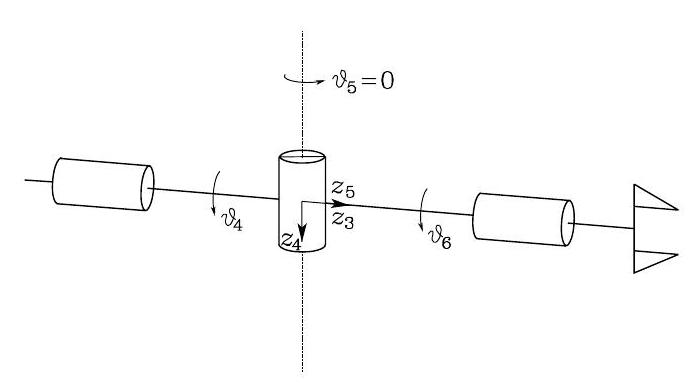
\includegraphics[max width=0.40\textwidth]{diff_kinematics/spherical_wrist_singularity}
    \caption{Spherical wrist at a singularity}
    \label{fig:enter-label}
\end{figure}




Wrist singularities can be determined by inspecting the block $\boldsymbol{\bar{J}}_{22}$. In fact, the wrist is at a singular configuration whenever the unit vectors $\boldsymbol{z}_{3}, \boldsymbol{z}_{4}, \boldsymbol{z}_{5}$ are linearly dependent. The wrist kinematic structure reveals that a singularity occurs when $\boldsymbol{z}_{3}$ and $\boldsymbol{z}_{5}$ are aligned, i.e., whenever

$$
\vartheta_{5}=0 \quad \vartheta_{5}=\pi
$$

The loss of mobility is  that the wrist is not allowed to rotate about the axis orthogonal to $\boldsymbol{z}_{4}$ and $\boldsymbol{z}_{3}$. 

\subsection{Arm Singularities}
Arm singularities are characteristic of a specific manipulator. To illustrate, consider the anthropomorphic arm.

\begin{figure}[H]
    \centering
    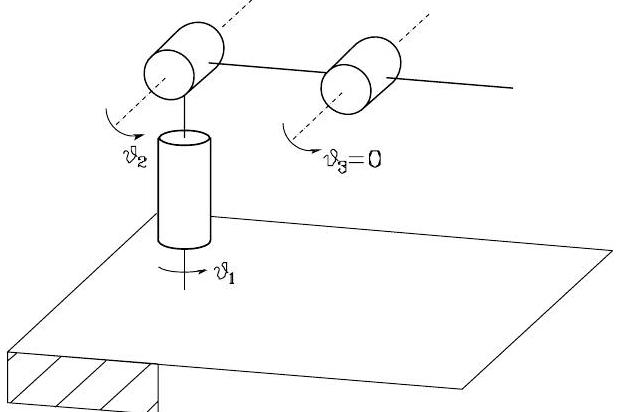
\includegraphics[max width=0.34\textwidth]{diff_kinematics/elbow_singularity.jpg}
    \caption{Anthropomorphic arm at an elbow singularity}
    \label{fig:enter-label}
\end{figure}


\begin{figure}[H]
    \centering
    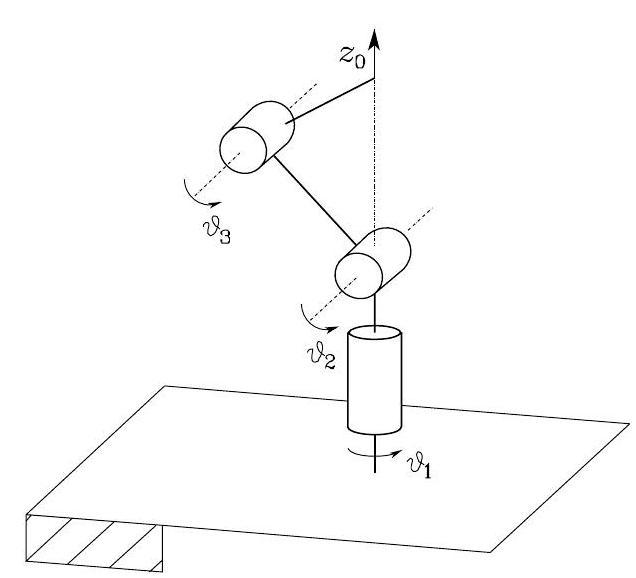
\includegraphics[max width=0.34\textwidth]{diff_kinematics/shoulder_singularity}
    \caption{ Anthropomorphic arm at a shoulder singularity}
    \label{fig:enter-label}
\end{figure}



 

The determinant of its Jacobian for the linear velocity part is 

$$
\operatorname{det}\left(\boldsymbol{\bar{J}}_{11}\right)=-a_{2} a_{3}  s_{3}\left(a_{2} c_{2}+a_{3} c_{23}\right)
$$


The determinant vanishes if $s_{3}=0$ or $\left(a_{2} c_{2}+a_{3} c_{23}\right)=$ 0. 


The case $s_{3}=0$ means that 

$$
\vartheta_{3}=0 \quad \vartheta_{3}=\pi
$$

meaning that the elbow is outstretched or retracted, and is termed elbow singularity. In this singularity, the loss of motion will be the linear motion along the direction of the third link (i.e., the direction perpendicular to $\boldsymbol{z}_2$ and $\boldsymbol{z}_0$.

The case $\left(a_{2} c_{2}+a_{3} c_{23}\right)=0$  means the wrist point lies on axis $z_{0}$, i.e., 

$$
p_{x}=p_{y}=0
$$

which is termed shoulder singularity. In this singularity, motions starting from the singular configuration that take the wrist along the $z_{1}$ direction are not allowed.



\section{Analysis of Redundancy}


The Jacobian describes the linear mapping from the joint velocity space to the end-effector velocity space, 

$$
\boldsymbol{v}_{e}=\boldsymbol{J}(\boldsymbol{q}) \dot{\boldsymbol{q}}
$$

where  $\boldsymbol{v}_{e}$ is meant to be the $(r \times 1)$ vector of end-effector velocity of concern for the specific task; $\dot{\boldsymbol{q}}$ is the $(n \times 1)$ vector of joint velocities; and $\boldsymbol{J}$ is the corresponding $(r \times n)$ Jacobian  that can be extracted from the geometric Jacobian. If $r<n$, the manipulator is kinematically redundant and there exist $(n-r)$ redundant DOFs.

\begin{figure}
    \centering
    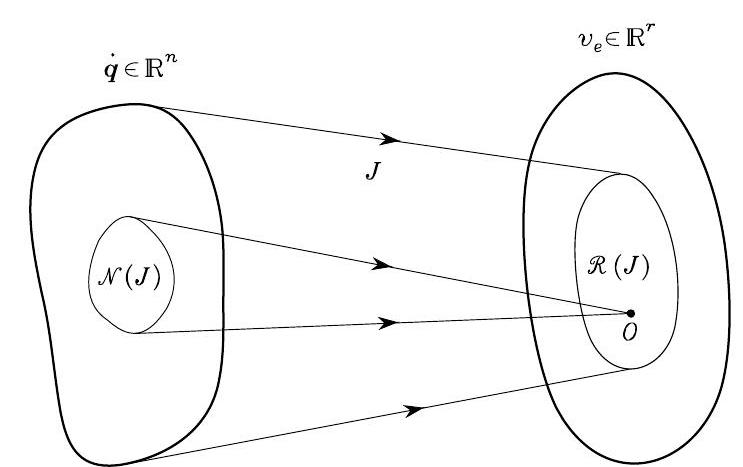
\includegraphics[max width=0.5\textwidth]{diff_kinematics/joint_to_operation.jpg}
    \caption{Mapping between the joint velocity space and the end-effector velocity space}
    \label{fig:enter-label}
\end{figure}

\begin{itemize}
  \item The range space of $\boldsymbol{J}$ is the subspace $\mathcal{R}(\boldsymbol{J})\subseteq \mathbb{R}^r$ of the end-effector velocities that can be generated by the joint velocities, given manipulator posture $\boldsymbol{q}$.

  \item The null space of $\boldsymbol{J}$ is the subspace $\mathcal{N}(\boldsymbol{J})\subseteq \mathbb{R}^n$  of the joint velocities that do not produce any end-effector velocity, given manipulator posture $\boldsymbol{q}$.

\end{itemize}

If the Jacobian has full rank, one has

$$
\operatorname{dim}(\mathcal{R}(\boldsymbol{J}))=r \quad \operatorname{dim}(\mathcal{N}(\boldsymbol{J}))=n-r
$$

and the range of $\boldsymbol{J}$ spans the entire space $\mathbb{R}^{r}$. Instead, if the Jacobian degenerates at a singularity, the dimension of the range space decreases while the dimension of the null space increases, since the following relation holds:

$$
\operatorname{dim}(\mathcal{R}(\boldsymbol{J}))+\operatorname{dim}(\mathcal{N}(\boldsymbol{J}))=n
$$

independently of the rank of the matrix $\boldsymbol{J}$

If $\mathcal{N}(\boldsymbol{J}) \neq \emptyset$, let $\boldsymbol{P}$ is a \emph{projection} $(n \times n)$ matrix so that

$$
\mathcal{R}(\boldsymbol{P}) \equiv \mathcal{N}(\boldsymbol{J})
$$

the joint velocity vector with arbitrary $\dot{\boldsymbol{q}}_{0}$

$$
\dot{\boldsymbol{q}}=\dot{\boldsymbol{q}}^{*}+\boldsymbol{P} \dot{\boldsymbol{q}}_{0}$$

is a solution to  $\boldsymbol{v}_{e}=\boldsymbol{J}(\boldsymbol{q}) \dot{\boldsymbol{q}}$. Here,
with $\dot{\boldsymbol{q}}^*$ a particular solution to $\boldsymbol{v}_{e}=\boldsymbol{J}(\boldsymbol{q}) \dot{\boldsymbol{q}}$. 

This result is of fundamental importance for redundancy resolution; it points out the possibility of choosing the vector of arbitrary joint velocities $\dot{\boldsymbol{q}}_{0}$ so as to exploit advantageously the redundant DOFs. 




\end{document}